\section{Discussion} \label{discussion-section}
\subsection{Conclusions}

\subsubsection{Focal unit: S\&P 500 versus Dow Jones Industrial}
Results of our analyses indicate that predominantly in the short term, there is a negative relationship between sentiment and subsequent stock returns of both \$SPY and \$DIA. \$SPY experiences the relationship in the shortest lags (1-week and 1-month). \$DIA shows more significant relationships with longer lags (6, 8 and 12 weeks). The effect sizes for these longer lags are also positive. In contrast, the significant results for \$SPY are prevalent in the shortest lags, although it does, as well, show significant relationships in some long term lags (6-week, 2-month and 3-month).
\par
Compared to previous research, Solt and Statman (1988) and Clarke and Statman (1998) investigated the connection between Investors Intelligence sentiment and DJIA and S\&P 500 returns for 4, 26 and 52-week lags. They did not find any significant relationship for either of the indices. In later research, Fisher and Statman (2000) investigate the influence of AAII investor sentiment on S\&P 500 subsequent returns with 1-month lag. They find negative relationship (<5\%) with slope of -0.10. Our findings are similar – negative slope of –0.15 at 5\% confidence level for S\&P 500 with one month lag. It is important to note that even though AAII reflects the investors opinion where the market will be in 6 months, our results are similar. By the velocity of posts and qualitative evaluation, we see that the investor sentiment on StockTwits has mainly short term focus. The number of messages sharply increases during higher market volumes which also highlights that the investors which share their sentiment on StockTwits are highly reactive. In contrary, Smales (2017) finds a positive slope (0.030) for AAII at 1\% and a negative (-0.086) slope at 1\% for VIX sentiment proxy. Fisher and Statman (2000) use data from 1987-1998 and Smales (2007) time-frame is 1990-2015 with 1-month lag. Our results, both significant and not significant exhibit positive relationship only in longer lags.

\subsubsection{Sentiment measure: Absolute versus Change}
The difference between change and absolute values in our research show that change in sentiments relates to longer lags. These outcomes (with longer lags – at least 2-month and 4-week) show positive relationship between sentiment and subsequent stock returns. Absolute sentiment measures show significant results in shorter term, which are mainly negative. 
\par
These findings again correspond with Fisher and Statman (2000). Change in the sentiment for individual investors, as well as newsletter writers, show a positive relationship (5\%) with a slope of 1.00 and 0.86, respectively. In Smales (2007), change in AAII produced positive slope, whereas change in VIX yielded negative results. This is consistent with the absolute measure as mentioned in the section above.
\par
Change of the investor sentiment is likely to show that a shift occurred which has implications to longer horizons, whereas the absolute values seem to be better in predicting the stock returns in near future. This logic would explain our results which are different for absolute and change in sentiment measures.

\subsubsection{Sentiment aggregate period and lags: Weekly versus Monthly}
The literature analysed uses mainly monthly periods since this choice is convenient as the investor sentiment was not measured that frequently. In our case, the novel approach to measuring investor sentiment provides us with larger amounts of data; thus, we can also investigate the hypotheses in weekly periods. Most of our significant results (10/14) measure the sentiment over weekly periods. This means that the investor sentiment obtained from social media and PsychSignal NLP algorithm is better in predicting shorter horizons. This is corresponding with the theory, since most of the StockTwits users are individual investors which tend to be more short-term focused and follow herd-like behaviour. This does not imply that the relationship is only in short term, though. The results show, that the sentiment is suitable for predicting also subsequent stock returns using longer lags. Short lags (1-week and 1-month) show negative relationship for both weekly and monthly periods. Longer lags exhibit more positive relationships. 

\subsubsection{Sentiment Measures} \label{sentiment-measure-discussion}
The direct StockTwits sentiment ("StockTwits") is significantly connected mainly to short term lags (1-week or 1-month). All relationships are negative, except monthly \$DIA (3-month lag) which has a positive relationship. The StockTwits sentiment indirectly estimated by PsychSignal ("PS:StockTwits") shows positive slope results in 3/5 significant instances. Overall, 17/32 tests (also non-significant at 10\%) show positive slope for PS:StockTwits investor sentiment and subsequent stock returns. This implies that the NLP algorithm for investor sentiment measure of StockTwits produces 47\% of all tests with a positive slope, whereas the direct measure provides only around 35\% of positive results. Only for significant results these numbers are 60\% and 25\%, respectively. When we look at the descriptive statistics, we see that PsychSignal data is more bullish than StockTwits direct measure. For both weekly and monthly data, the bullish mean percentage is 0.60 for PsychSignal databases ("PS:StockTwits" and "PS:Aggregated") and 0.42 for StockTwits. This contributes to the fact that the results of the tests using PsychSignal NLP databases show higher percentage of positive results.
\par
There are no significant results between StockTwits and PS:StockTwits which have the same properties (period, time lag, focal unit) so we cannot compare the two sentiments’ predictive power exactly. However, for 1-month and 1-week lags, both measures show negative relationship to subsequent sentiment measures. The positive significant results are connected to longer lags – this applies mainly to PsychSignal investor sentiment measures.
\par
The sentiment from aggregated dataset ("PS:Aggregated" - Twitter and StockTwits indirectly measured by PsychSignal) never shows a significant relationship for monthly measures. On the other hand, the significant results (<10\%) obtained from this sentiment measure have at least 6-week lag.
\par

\subsubsection{Results Synthesis: Patterns in Results}
How do all these insights come together? For S\&P 500 both weekly and monthly directly measured absolute investor sentiment ("StockTwits") for 1 period lags show significant negative slope of -0.0328 and -0.1531, respectively. DJIA follows this pattern too - for the weekly sentiment absolute measure ("PS:StockTwits") the slope is -0.0339. These findings match with the previous research. 
\par
When we enter the questions about shorter versus longer lags, absolute versus change and monthly versus weekly sentiment aggregates, the results are more complex. In general, shorter lags seem to exhibit mainly negative effect sizes and longer lag periods have mainly positive relationship towards subsequent stock returns. The exception is a lag of 6 weeks, which has all significant relationships negative for both S\&P 500 and DJIA using the aggregated investor sentiment.
\par
The positive relationships only apply to the DJIA index with one exception: S\&P 500 monthly, absolute, 3-month lag, "PS:StockTwits". This is the longest lag with monthly sentiment measure period and it has a positive effect size even for S\&P 500. It seems that in long run, the investor sentiment is indeed positively connected to subsequent stock returns both in DJIA and S\&P 500 indices. This effect is more prevalent for DJIA; this index exhibits the positive relationships also for weekly periods.
\par
It appears that in the short term and for a more diverse portfolio (S\&P 500), the investor sentiment decreases subsequent stock returns; however, in the long run and with a portfolio of large, traditional companies (DJIA), the relationship seems to shift towards the positive. This likely shows that investors' positive view of the future returns is fulfilled for large, traditional companies which are in Dow Jones Industrial Average. In contrast, for S\&P 500, the overreaction of investors allows arbitrageurs to drive stock prices back to equilibrium. This is congruent with the fact that most StockTwits users are individual investors and thus likely targets for more professional investors. This effect can be seen in Figure~\ref{fig:excelbars}, where all the tests are summarized. Both for significant and not significant results, the effect sizes are positive as the lags are getting longer. In first column, the label for the test is specified. The bars show the magnitude of the relationship and the colour shows the significance. The vertical lines show the recurring lag periods (1, 4, 6 and 12 weeks, and 1, 2 and 3 months). 

\newpage
\begin{figure}[h]
\centering
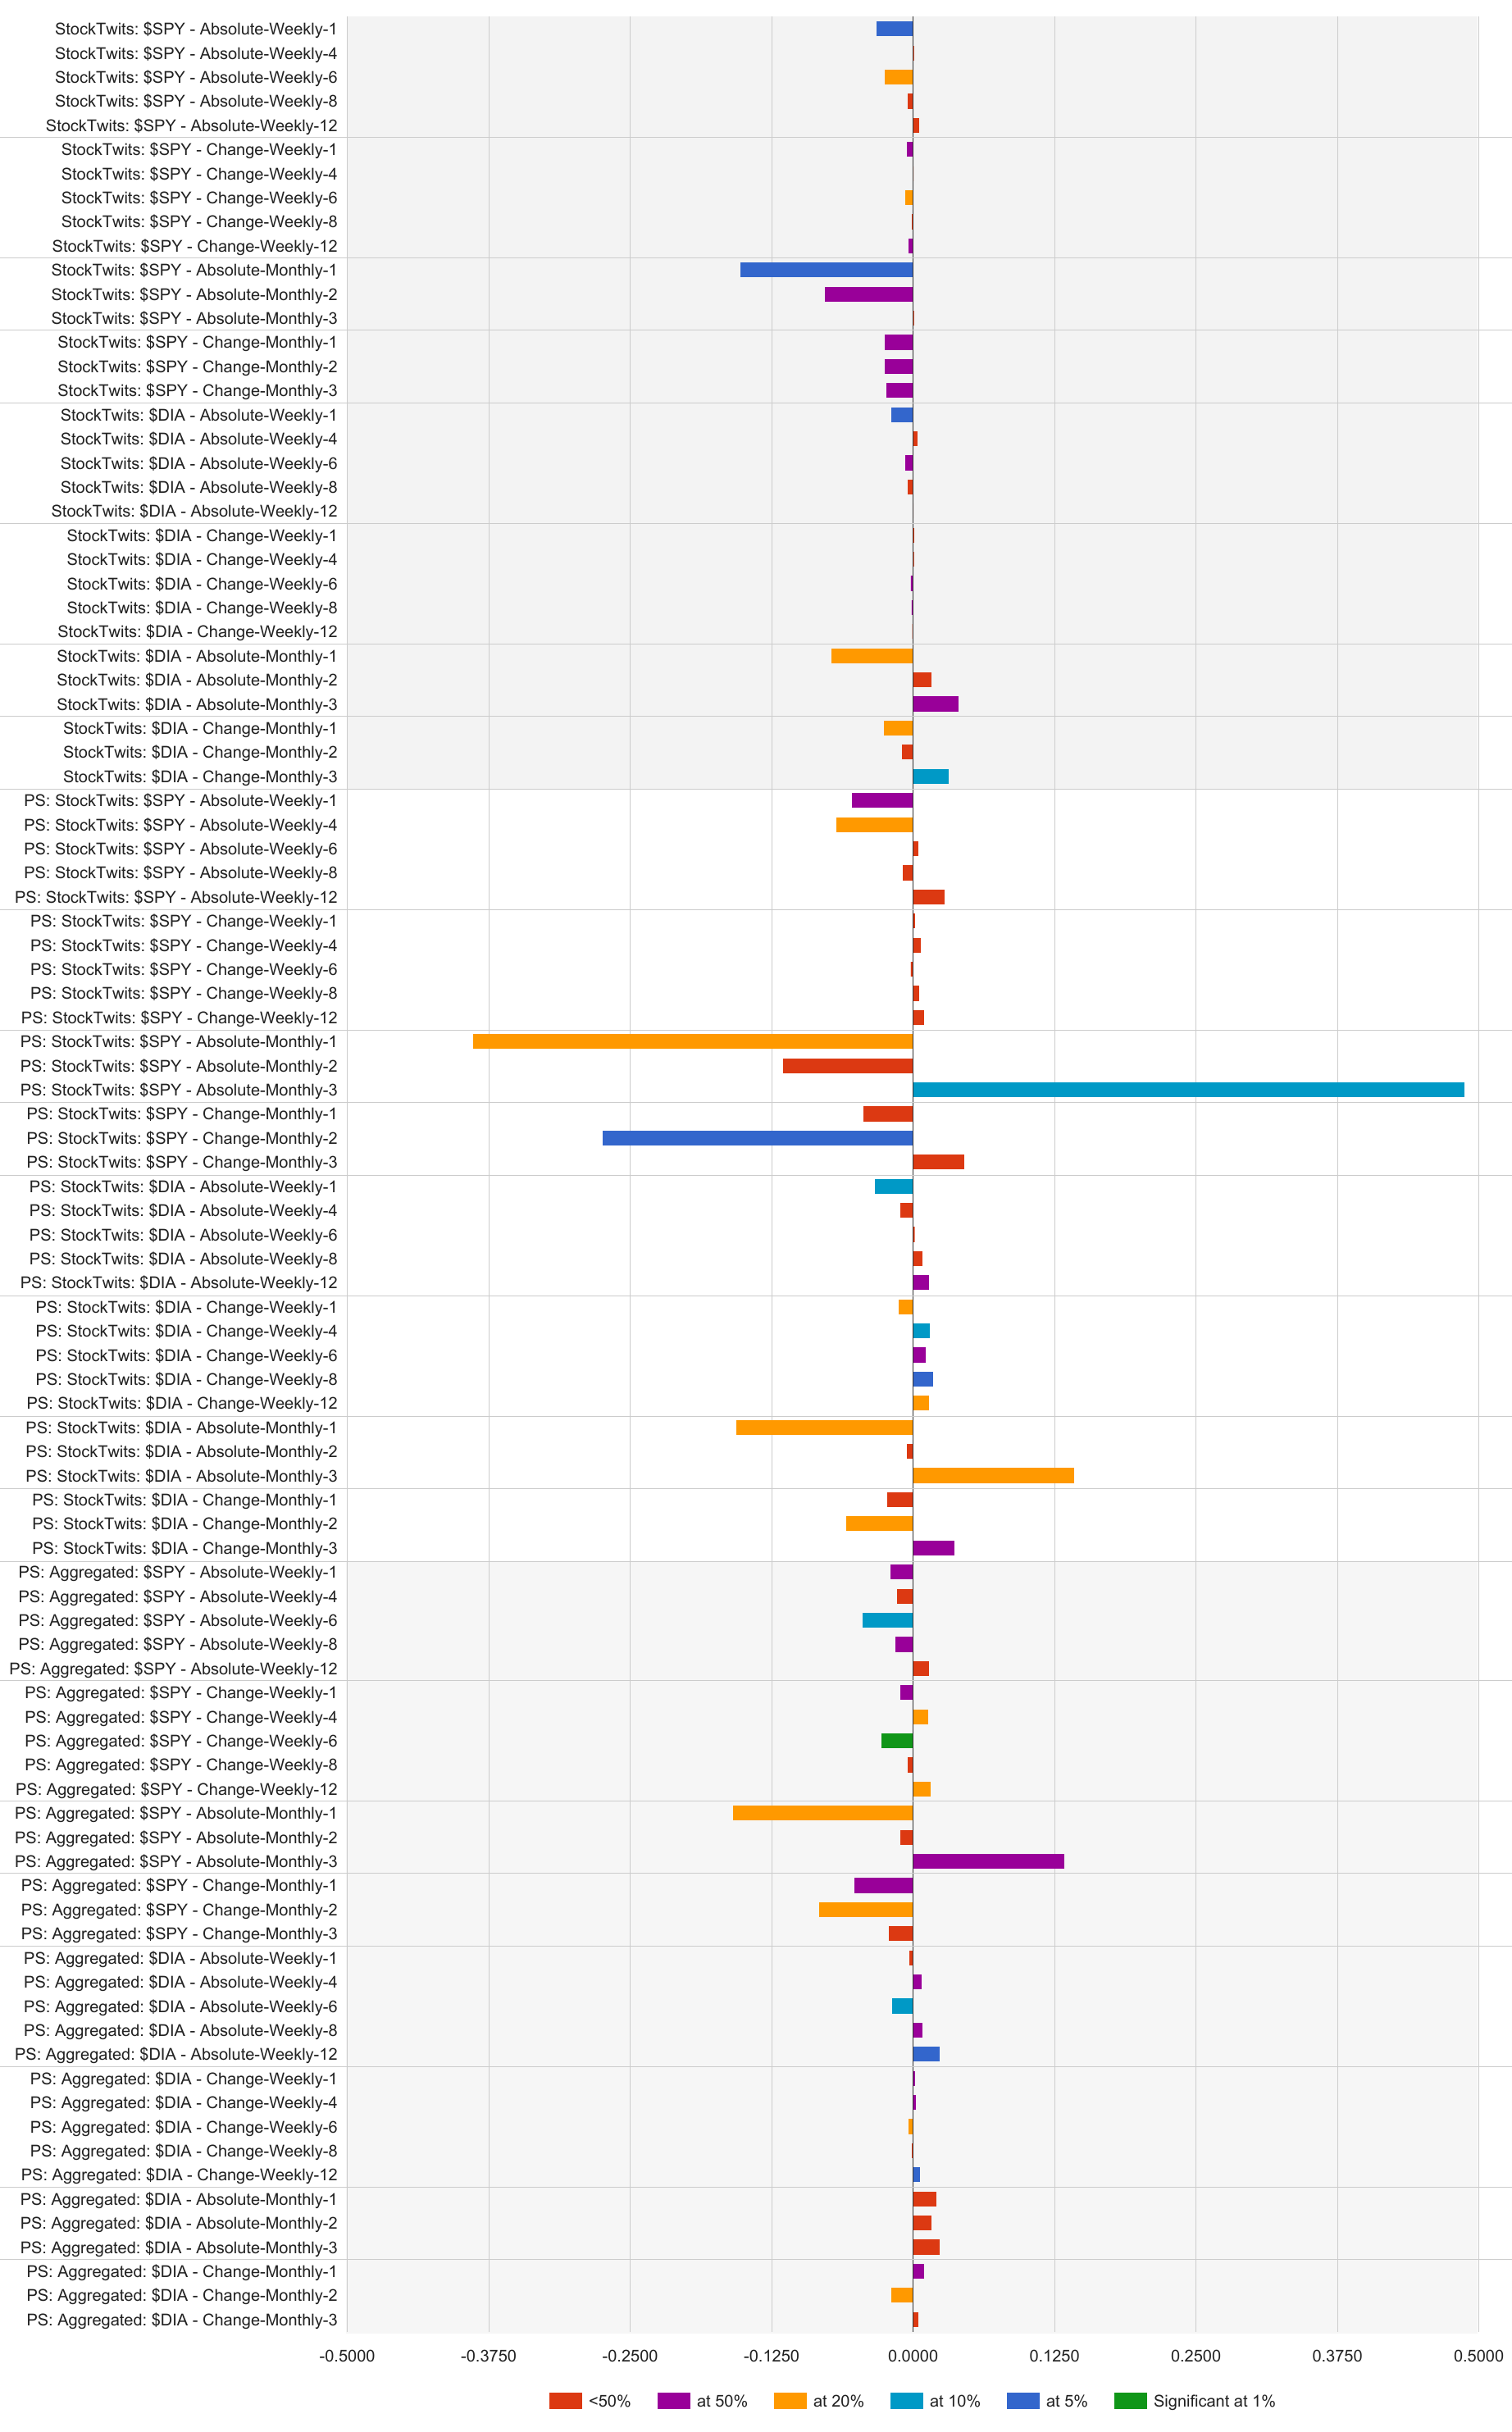
\includegraphics[width=.95\textwidth]{figures/sickExcelBars.png}
\caption{\label{fig:excelbars}Effect sizes of the regressions and their significance}
\end{figure}

\subsubsection{Economic Significance}
The effect sizes of most of our results are that 1\% change or increase of 1 in investor sentiment yields to sub 0.10\% change in stock returns. The exact magnitudes can be seen in Figure~\ref{fig:excelbars}. These results are similar to the results of Smales (2017) for large caps, Brown and Cliff (2002) for smaller companies and Fisher and Statman (2000) for individual investors sentiment on S\&P 500. There are no clear patterns in the magnitudes of our results and the results of past papers. Including the sentiment measures that we explored in our research, would therefore be a good addition to other tools when deciding on an investment, rather than a single decisive factor. The largest application of our findings are most suitable to quantitative trading, where it will help to fine tune the algorithms. 

\subsection{Recommendations}
Our aim was to investigate these new, modern sentiment measures and their relationship to subsequent stock returns. The services which gather and compile the sentiment measures (StockTwits and PsychSignal) create large datasets which are publicly available for people to use in their research or investment strategy. Investors can employ our findings in multiple ways. When constructing an algorithmic trading strategy, they can include a variable which tracks the sentiment measure either from PsychSignal or StockTwits and improve their predictive power of subsequent stock returns.

\subsection{Limitations and Future Research}
Since NLP processing and trading social networks such as StockTwits are fairly new concepts, we have analysed only the recent years (2014-2016) since this is the period for which the number of investor sentiment measures is sufficient to perform this type of research. This also prevented us from using a company level approach as desired from the start. As a proxy for returns of S\&P 500 index returns, we employed the S\&P 500 ETF \$SPY since this was the only data available to us on the research platform Quantopian where we accessed the PsychSignal databases. The velocity of the data is insufficient (so far!) to perform a company level (stock by stock) analysis for all S\&P 500 stocks on the effect of this type of investor sentiment on subsequent stock returns. When investigating the data, we have seen a huge growth over the recent years and we strongly believe that company level analysis will be available in the near future. This is also related to the decision to use aggregated data over weeks and months. Larger amounts of data will allow researchers to investigate these relationships on a day-to-day basis with sufficient data for either S\&P 500 or all stocks in NASDAQ or NYSE. We consider that shorter lags used in the upcoming research would bring more insights into how fast the social media investor sentiment can affect the subsequent stock returns.
\par
Furthermore, we tried to also test aggregating all daily sentiment (for all stock symbols) in StockTwits database and regressing this variable on Dow Jones Industrial Average and S\&P 500 indices. These tests did not yield any significant results and most of the p-values were higher than 0.90 for all lags. This big data approach is likely to become more relevant as more sentiment data will be generated by the users, both on Twitter and StockTwits.
\par
Regarding the absolute investor sentiment measures, some argue that causality in this measure is lowered as the effect size parameter may not be the correlation or regression of changes of investor sentiment on changes of stock returns, but may be the correlation or regression of the values of these variables at different points in time. This changes the quasi-experimental approach to a cross-sectional study over time, which means that causal inferences are not strictly implied.
